\documentclass[10pt, a4paper]{article}

\usepackage{simplecv}
\usepackage{pdfpages}
% to see the layout, you can uncomment these lines

%\usepackage{showframe}
%\renewcommand\ShowFrameLinethickness{0.15pt}
%\renewcommand*\ShowFrameColor{\color{red}}
% \usepackage {xcolor}

\begin{document}

	\name{ Sajed Zarinpour Nashroudkoli}
	\contactInfo
	{Tehran, Tehran, Iran}
	{ +98-935-218-8208 }
	{sajed.zarinpour@gmail.com}
	{https://www.linkedin.com/in/sajed-zarinpour}

	\section*{Education} 
		\eduEntry
		{{Sep. 2017\\Oct. 2020} \hspace{.5em}\normalsize}
		{M.Sc. in Applied Mathematics}
		{Institute for Advanced Studies in Basic Sciences, Iran}
		{Numerical Method for Solving PDEs with Uncertainty Using Neural-Network}
		{ 
			\explist{
				Implemented a new layer for padding inputs using tf \href{https://github.com/sajed-zarrinpour/Solving-PDE-with-Uncertainty-surrogate-forward-model-keras/blob/master/NLSE/NLSE2D.ipynb}{[GitHub Repo]}; 
				Gained extensive knowledge on biophysical models
			}
			\skills{Python, Numpy, Bash, TensorFlow, Keras, Matplotlib, Octave, Latex} 
		}
		
		\eduEntry
		{\small{Sep. 2012\\Sep. 2017}\hspace{.5cm}}
		{B.Sc. in Applied Mathematics}
		{University of Guilan, Iran}
		{Study on GMDH Algorithm for Stock Price}
		{ 
			\explist{
				Represented a novel definition for Graphs to solve recursive problems including conditional based actions to solve NP-hard partition problem \href{https://github.com/sajed-zarrinpour/Number-Partitioning/blob/master/Graph.md}{[GitHub]}
			}
			\skills{MATLAB (Octave), C++}
		}
	
	\section*{Skills}	
	\aside
	{
		\bold{Comupter Skills}
	}
	{
		\skills
		{
			Linux,
			Python,
			TensorFlow,
			Keras,
			Numpy,
			Pandas,
			MATLAB,
			NgSolve,
			git,
			Freefem++,
			C++,
			Julia,
			RDBMS,
			LaTeX
		}
	}
	\aside
	{
		\bold{Soft Skills}
	}
	{
		\skills
		{
			Teamwork,
			Stress Management,
			Innovation
		}
	}
	
	\section*{Research \& Interests}
	\interestslist
	{
		% research and interests
		Mathematical Modeling,
		Biological Systems,
		Finite Element Method, 
		Numerical Analysis,
		Deep Learning,
		Inverse Problems
	}

		
	\section*{Experiences}

		\expEntry
		{Apr. 2024\\Present}
		{Senior Web Developer}
		{Islamic Azad University Electronic Campus}
		{Tehran}{}
%		{\textcolor{gray}{\skills{Laravel, Moodle, PHP, MySQL, Linux}}}

		\expEntry
		{Dec. 2023\\March 2024}
		{Web Developer}
		{Motegharen}
		{Rasht}{}
%		{\textcolor{gray}{\skills{Laravel, Rest API}}}
	
		\expEntry
		{Jan. 2021\\Nov. 2023}
		{Conscription}
		{Iranian Traffic Police}
		{Tehran}{}
	
		\expEntry
		{Dec. 2020\\Nov. 2021}
		{Database Analyst / Developer}
		{Tavana System}
		{Zanjan}{}
%		{\textcolor{gray}{\skills{Python, Microsoft SQL server, Slack}}}
		
	\section*{Schools \& Conferences}
		
		\confEntry{2020}{ IASBS Student Presentations in English \\ \normalfont \skills{Presented: On Solving Partial Differential Equations using Neural Networks} }{ Institute for Advanced Studies in Basic Sciences }	
	
%		 \centerline{***} 
%		\slimseperator
		
		\confEntry{2021, 2024}{ Population Dynamics }{ Jena University }

		\confEntry{2021}{ An Introduction to Variational Analysis (Summer School) }{ Miami University, Urmia University of Technology }
		
		\confEntry{2020, 2021}{ One World IMAGINE seminars }{ Siam }
		
		\confEntry{2020}{ Solving inverse problems with deep learning }{ UC Berkeley Applied Math Seminar }
		
		\confEntry{2019}{ Introduction to Data Science in R }{ Institute for Advanced Studies in Basic Sciences }
		
		\confEntry{2019}{ From Biophysical Modeling to Simulation Codes (Winter School) }{ Graz university, Isfahan University of Technology }	
	
	\section*{Languages}
	
	\languageEnry{ \textbf{English}}{ Upper Intermediate} Listening C1, Reading B2, Spoken Interaction C1, Spoken Production C1, Writing C1
	\small (According to \href{https://europass.cedefop.europa.eu/resources/european-language-levels-cefr}{European language levels}: Basic user (A1, A2) - Independent user (B1, B2) - Proficient user (C1, C2))\\
%	\selfAssessedEng{C1}{B2}{C1}{C1}{C1} % Listening, Reading, Spoken Interaction, Spoken Production, Writing
	
	\languageEnry{\textbf{German}}{(Beginner)} % Listening A1, Reading A1, Spoken Interaction A1, Spoken Production A1, Writing A1 \\\\

	\section*{References}
%		Available on Request
	\refEntry{(M.Sc. Supervisor)}{Dr. Khadijeh Nedaiasl}
{Assistant Professor of Applied Mathematics}
{nedaiasl@iasbs.ac.ir} %(+98) · 24 · 3315 · 5053
{IASBS, mathematics department}

\refEntry{(M.Sc. Advisor)}{Dr. Parvin Razzaghi}
{Assistant Professor of Computer Science and Information Technology}
{p.razzaghi@iasbs.ac.ir} %(+98) · 24 · 3315 ·3375
{IASBS, computer science and information technology department}

%	\headline{Cover Letter}
	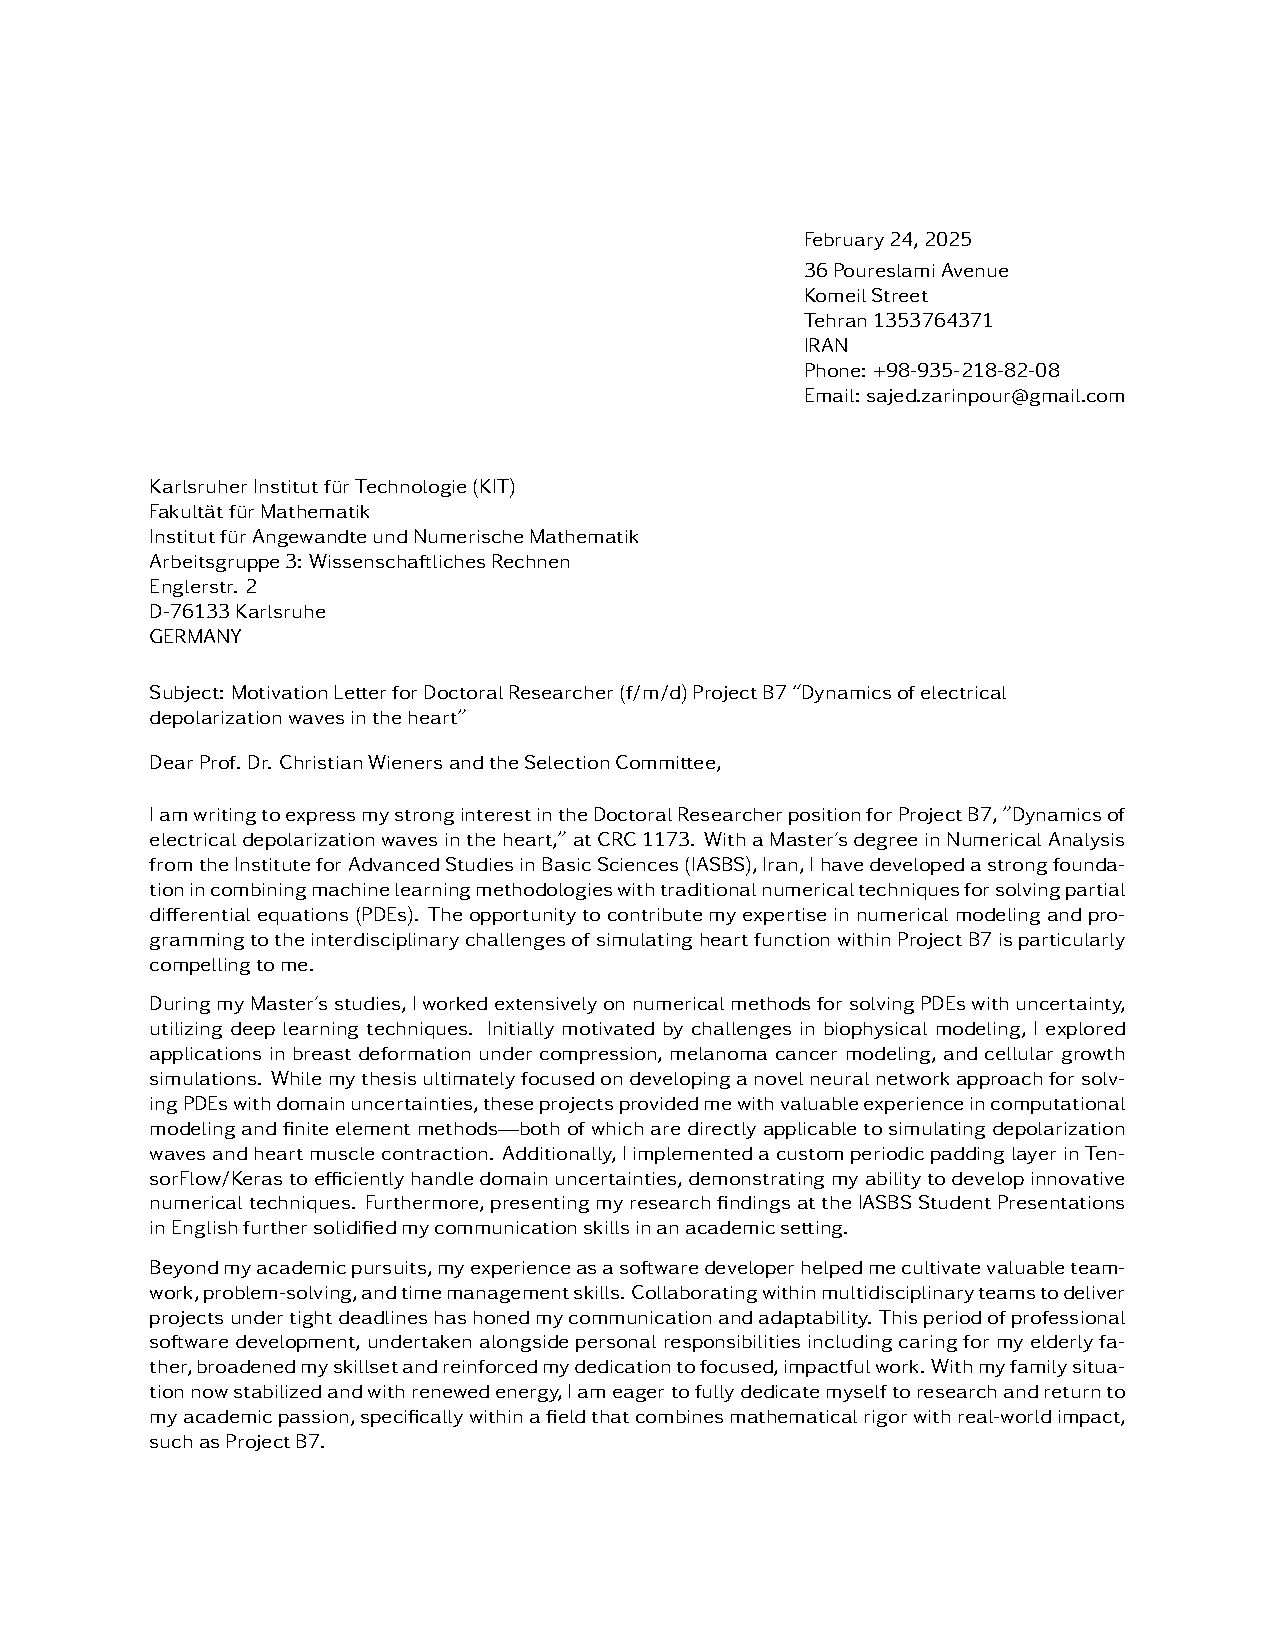
\includepdf[pages=-]{CoverLetter/cover_letter_sajed_zarinpour.pdf}

		\headline{ Statement of Research}
	
	\section*{Introduction}
	The convergence of numerical analysis, deep learning, and biological systems presents a fertile ground for addressing complex phenomena governed by partial differential equations (PDEs). Project B7, "Dynamics of electrical depolarization waves in the heart," within the Collaborative Research Center (CRC) 1173, offers a compelling opportunity to contribute to this interdisciplinary domain. Specifically, the project's focus on accurately simulating cardiac depolarization while accounting for the dynamic deformations of the heart muscle poses a significant computational challenge, necessitating the development of advanced numerical methodologies. This research aims to advance the state-of-the-art in cardiac modeling by integrating established numerical techniques with innovative machine learning approaches.
	\section*{Previous Research Experience}
	My graduate research at the Institute for Advanced Studies in Basic Sciences (IASBS) centered on the development and application of neural network-based methodologies for solving PDEs with uncertainty. This research involved the synthesis of deep learning techniques with classical numerical methods, resulting in the creation of a novel computational framework. A key contribution was the implementation of a custom periodic padding layer within the TensorFlow/Keras environment, designed to efficiently manage domain uncertainties. This experience provided a robust foundation in numerical algorithm development and implementation, alongside proficiency in Python, TensorFlow/Keras, and related computational tools. Furthermore, the initial motivation for this research stemmed from biophysical modeling challenges, including simulations of breast deformation, melanoma cancer modeling, and cellular growth, which fostered a keen interest in applying advanced computational techniques to biological systems.
	\section*{Research Goals}
	The overarching research objective within Project B7 is to contribute to the development of sophisticated mathematical models for cardiac depolarization, explicitly incorporating the intricate dynamics of heart muscle contraction. This will involve extending and refining existing modeling paradigms within the CRC, leveraging recent advancements in biophysical understanding.
	
	A central component of this research will be the utilization of the CRC's M++ finite element system to generate initial solution frames. Given the computational demands associated with simulating dynamic cardiac deformations, I propose to integrate physics-informed neural networks to learn and refine these initial solutions. By training neural networks on the output of M++ simulations, a hybrid methodology will be developed, synergistically combining the accuracy of finite element methods with the efficiency and adaptability of deep learning. This approach will enable the capture of the complex spatiotemporal dynamics of depolarization waves, enhancing the fidelity of cardiac simulations.
	
	Specifically, the research will focus on:
	\begin{itemize}
		\item The development of hybrid numerical schemes that seamlessly integrate M++ simulations with neural network-based refinement.
		\item The application of physics-informed neural networks to learn the underlying biophysical principles of cardiac depolarization, thereby improving the accuracy of time-dependent simulations.
		\item The exploration of efficient interpolation and extrapolation techniques to generate high-resolution simulation data from learned neural network representations.
	\end{itemize}
	
	Ultimately, this research aims to develop robust and scalable computational tools that will advance our understanding of cardiac function and contribute to the overarching objectives of Project B7 and CRC 1173. The interdisciplinary nature of this endeavor, facilitating collaboration between mathematicians and biomedical engineers, is particularly compelling.
		
\end{document}
